\section{Project guidelines}
\subsection{Deployment plan}
\subsubsection{Scheduling and Timeframes}
   
\begin{center}
    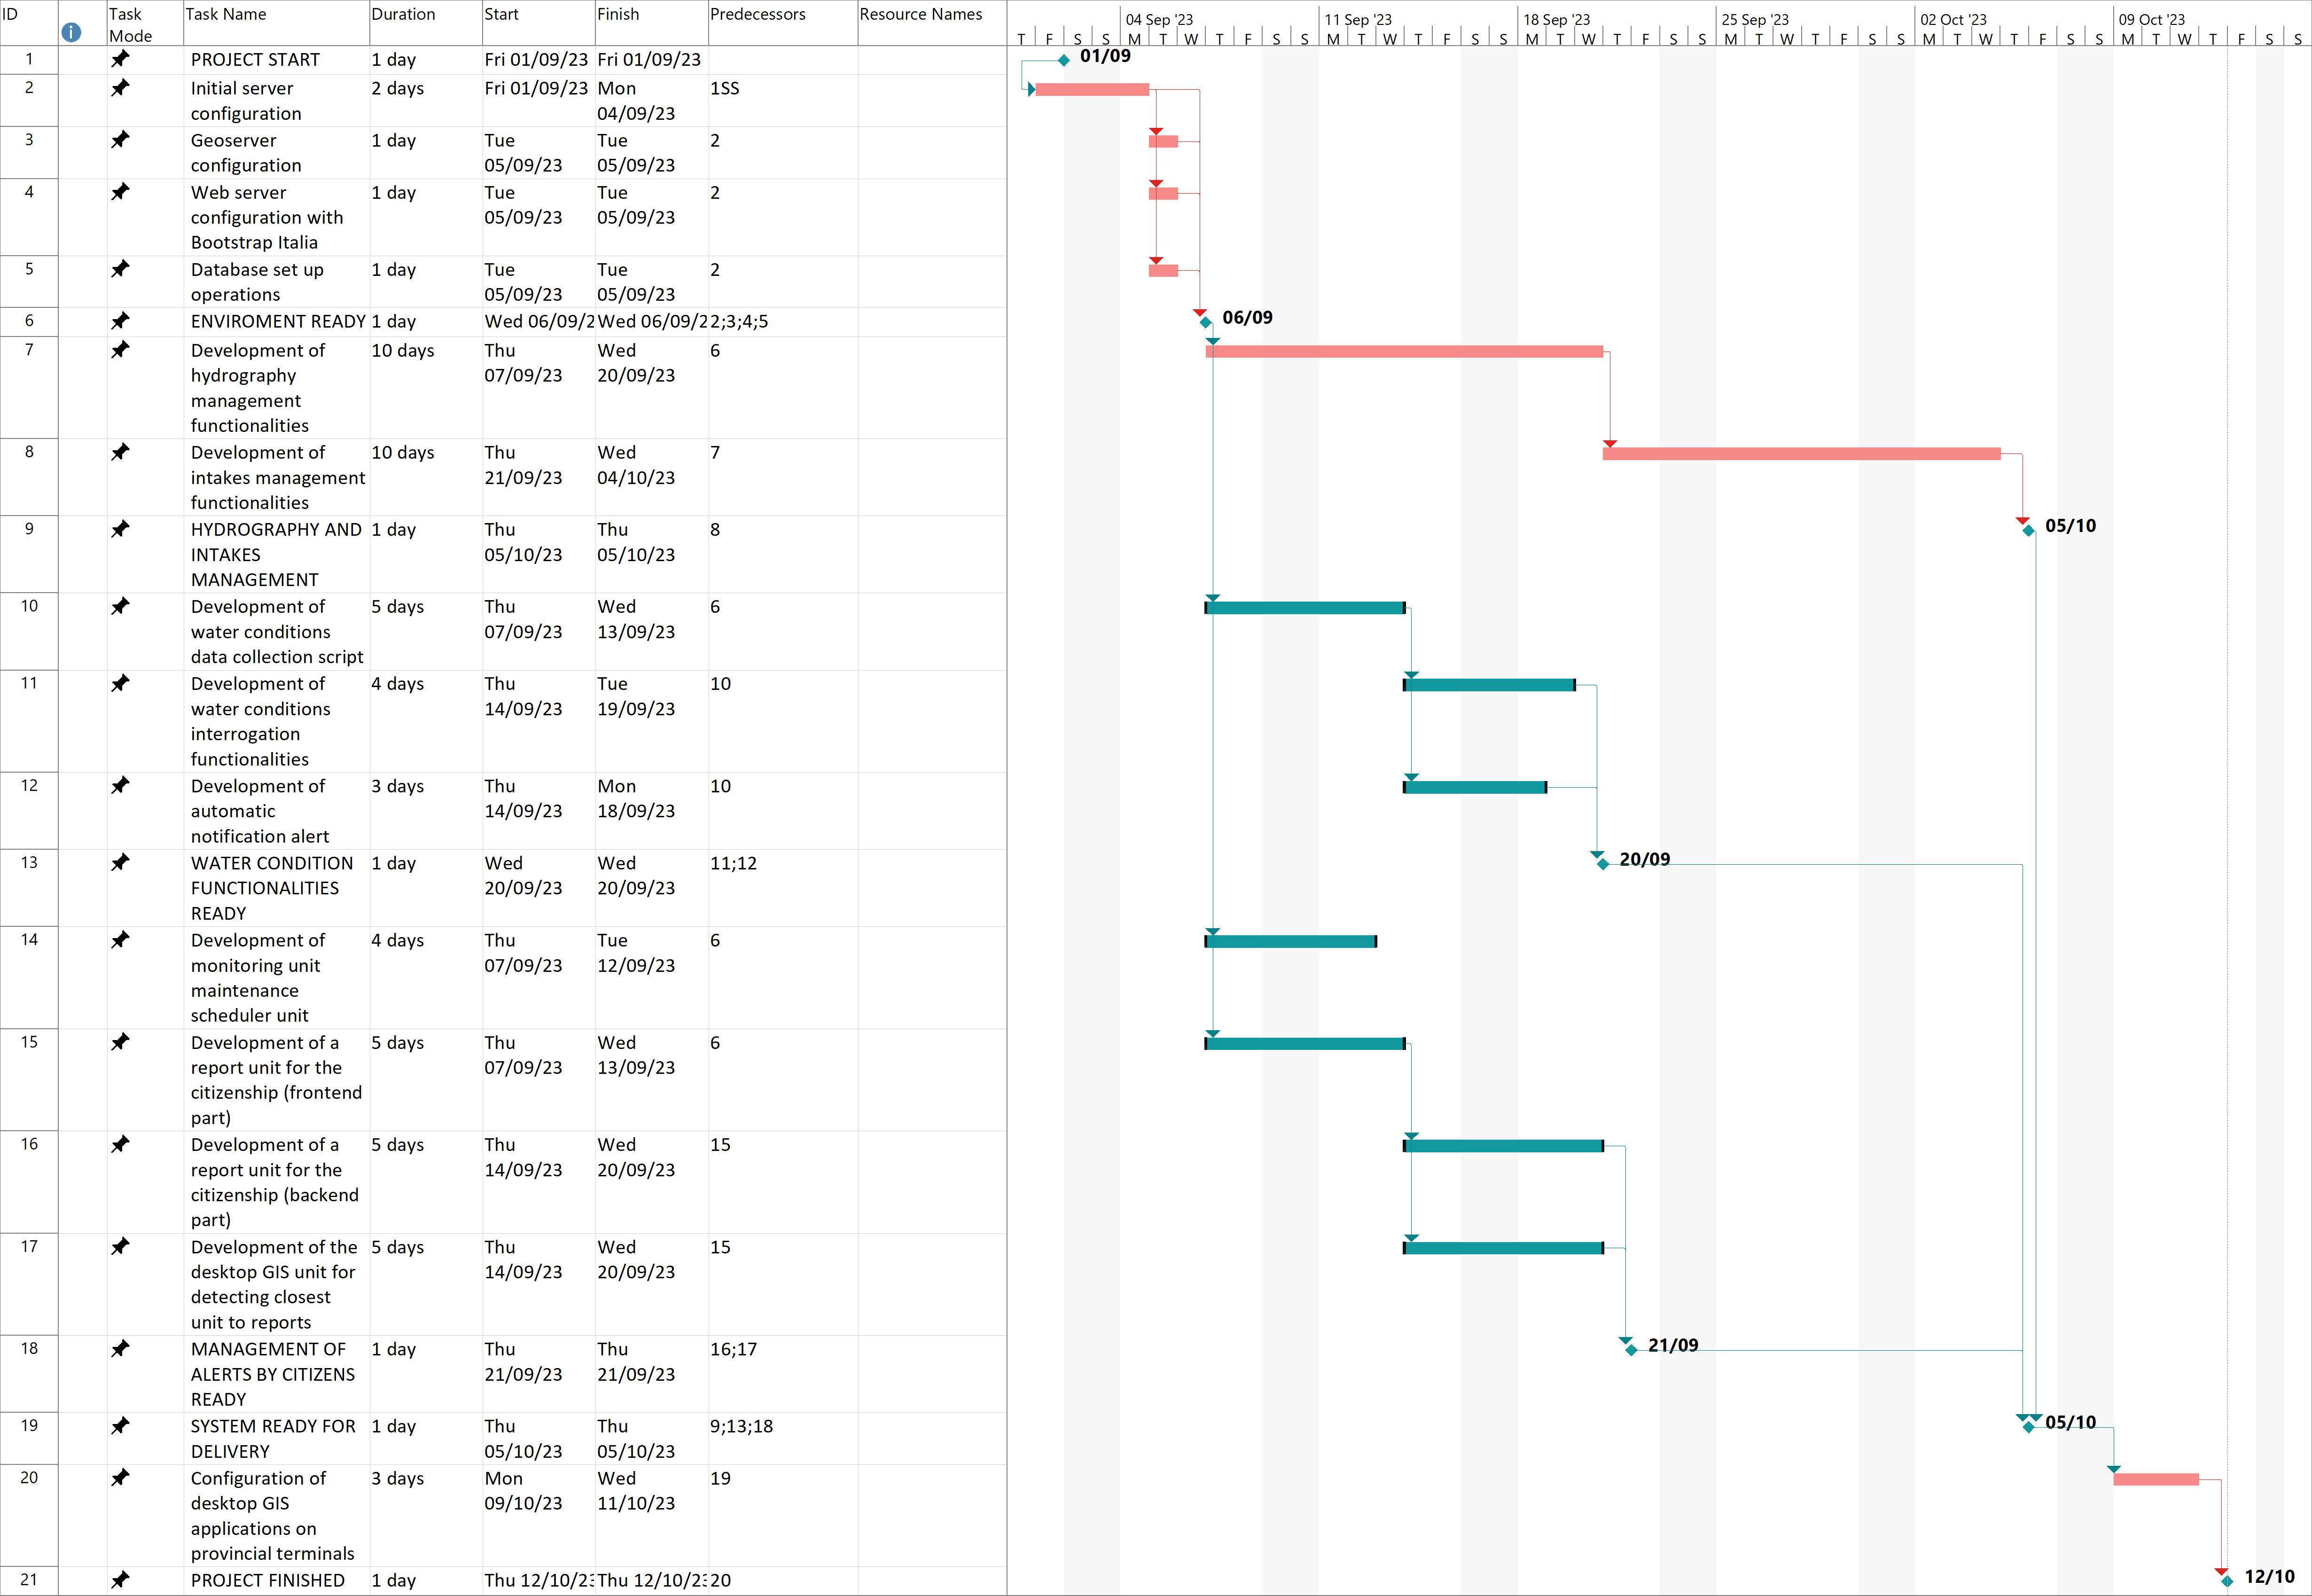
\includegraphics[width=\textwidth]{img/gantt.png}
\end{center}

\subsubsection{Description}
In the Gantt chart are shown all the activities necessary to reach the final goal; the working hypotesis is to start the project by the 1st of September 2023 with the sever configuration procedures and then finish up everything (if no delays happens) by the 12th of October: the whole execution then should take around one month and a half.
This hypotesis does not take care of the number of working resources (software engineers or programmers) available for the execution, that can led to a more constrained execution due to many parallelized activities. \\
Activities coloured in pink represents the \textit{critical path}, that are the ones in which a delay can led to a delay of the whole project.

\subsubsection{Deliverables}
From the Gantt chart is visible that three main milestone are present in the timeline of the project: these coincides with three different \textit{deliverables}, that are three tangible and atomically usable parts of the system.\\
In particular:
\begin{itemize}
    \item \textbf{05/10}: this milestone coincides with the delivery of the hydrography and intakes management functionalities. Theoretically, from this date the provincial emplyees can start to use and to test this subpart of the system;
    \item \textbf{20/09}: this milestone coincides with the delivery of the automatic data reading subsystem from the web gateways and the email alert system. Theoretically, from this date the provincial emplyees can start to use and to test this subpart of the system;
    \item \textbf{21/09}: this milestone coincides with the delivery of the reporting subsystem for the citizenship and its backend and desktop management functionalities. Theoretically, from this date the provincial emplyees can start to use and to test this subpart of the system.
\end{itemize}

\subsection{Risk management}
Many activities can be conducted to study risks in a project. One possible approach can be to conduct a \textit{FMEA} analysis, but the size of the actual project is not so big to justify such an extensive analysis. \\
A better approach for the actual project has been found in filling a risk register.

\subsubsection{Risk matrix}
To evaluate the level of a risk (in a scale of three levels, \textit{low}, \textit{medium} and \textit{high}) we can use the risk matrix that is defined as follows:
\begin{table}[H]
    \centering
    \begin{tabular}{|cc|c|c|c|}
    \hline
    \multicolumn{2}{|l|}{\textbf{IMPACT}}                      & Low    & Medium & High   \\ \hline
    \multicolumn{1}{|l|}{\multirow{3}{*}{\rotatebox{90}{\textbf{PROB.}}}} & High   & \cellcolor{orange!25}Medium & \cellcolor{red!25}High & \cellcolor{red!25}High   \\ \cline{2-5} 
    \multicolumn{1}{|l|}{}                   & Medium & \cellcolor{green!25}Low    & \cellcolor{orange!25}Medium & \cellcolor{red!25}High   \\ \cline{2-5} 
    \multicolumn{1}{|l|}{}                   & Low    & \cellcolor{green!25}Low    & \cellcolor{green!25}Low    & \cellcolor{orange!25}Medium \\ \hline
    \end{tabular}
\end{table}

\subsubsection{Risk register}
\begin{table}[H]
    \centering
    \begin{tabularx}{\columnwidth}{|X|X|X|c|c|c|c|}
    \hline
    \textbf{DESCR.} & \textbf{CAUSE} & \textbf{DAMAGE} & \textbf{PROB.} & \textbf{IMPACT} & \textbf{LEVEL} & \textbf{ACTION} \\ \hline
    Data breach & Malicious intrusion with the purpose of steal data & Sensible data exiting from the system & \cellcolor{green!25}L & \cellcolor{orange!25}M & \cellcolor{green!25}L & Mitigate \\ \hline
    Denial of service & Malicious will of attackers of blocking the system & Unavailability of the system & \cellcolor{green!25}L & \cellcolor{red!25}H & \cellcolor{orange!25}M & Mitigate \\ \hline
    Monitoring unit malfunctioning & Broken sensor (not detected) that returns uncorrect data & Uncorrect alerts sent by mail & \cellcolor{green!25}L & \cellcolor{red!25}H & \cellcolor{orange!25}M & Transfer \\ \hline
    Impossibility of data acquisition & Unit readings not returned due to mobile network malfunctions & Missing pollutants monitoring in a certain unit of time & \cellcolor{green!25}L & \cellcolor{red!25}H & \cellcolor{orange!25}M & Transfer \\ \hline
    Fake reporting & Malicious will from citizens to report unreal alterations & Untrustable data & \cellcolor{orange!25}M & \cellcolor{orange!25}M & \cellcolor{orange!25}M & Accept \\ \hline
    \end{tabularx}
\end{table}

\subsection{Benefits evaluation}
\subsubsection{Benefits identification}
By analyzing the system's functionalities and capabilities, we identify the following benefits:
\begin{itemize}
    \item Fast water pollution detection and circumscription: in case of polluting events, by the alert system is possible to isolate the pollutants quickly, contacting the authorities and avoiding costly reclaim activities;
    \item Transparent governance: the dedicated portal for water quality analysis results and the citizen reporting system will promote transparency in governance. Citizens will actively participate in the supervision of the province's water heritage by reporting incidents and alterations, fostering a sense of responsibility and engagement in environmental protection;
    \item Data-driven decision making: The system's capabilities for querying and visualizing data will provide valuable insights for informed decision-making. By analyzing historical data and monitoring trends, the province can proactively address water-related challenges, implement preventive measures, and optimize resource allocation;
    \item Improved efficiency and data accessibility: with the implementation of a user-friendly WebGIS application and advanced querying capabilities, accessing and retrieving hydrography data will become more efficient and streamlined. Technical offices and authorized personnel will have real-time access to essential information, reducing response times for critical interventions;
    \item Compliance with standards and regulations: through adherence to relevant hydrography management standards and regulations, the system will ensure that the province's water management practices align with national and international guidelines. This compliance will enhance the province's reputation and bolster its commitment to responsible water resource management.
\end{itemize}

\subsection{Economic quantification of the benefits}
